\documentclass[crop,tikz]{standalone}
\usepackage{tikz}
\usetikzlibrary{arrows.meta, positioning, shapes, backgrounds}

\definecolor{deepblue}{RGB}{10,40,130}
\definecolor{darkteal}{RGB}{0,90,90}
\definecolor{richorange}{RGB}{230,90,10}
\definecolor{plumpurple}{RGB}{90,10,150}

\begin{document}
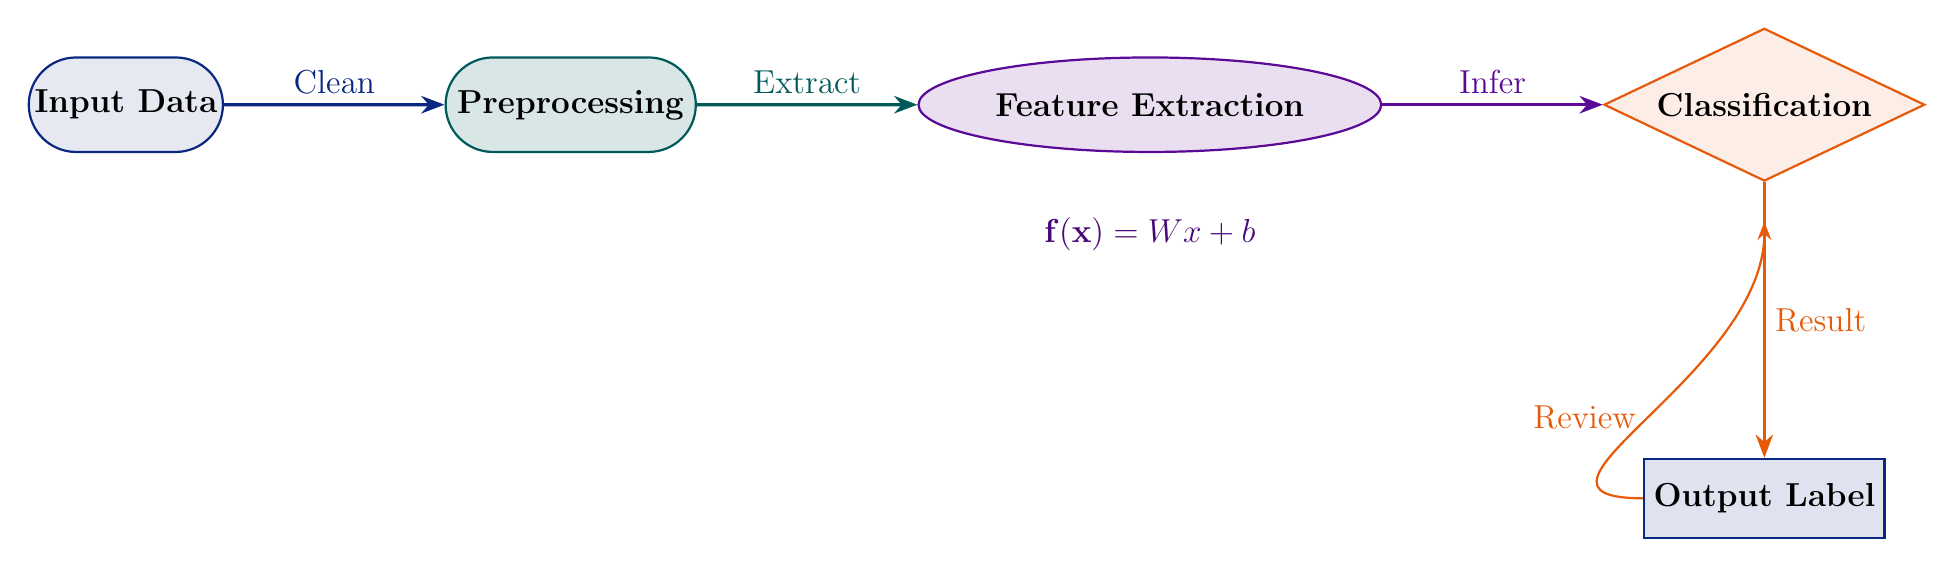
\begin{tikzpicture}[node distance=3.5cm and 2.8cm, font=\large, >=Stealth]

% Nodes
\node[rounded rectangle, draw=deepblue, thick, fill=deepblue!10, minimum width=2.7cm, minimum height=1.2cm] (start) {\textbf{Input Data}};
\node[rounded rectangle, draw=darkteal, thick, fill=darkteal!15, minimum width=2.7cm, minimum height=1.2cm, right=of start] (preprocess) {\textbf{Preprocessing}};
\node[ellipse, draw=plumpurple, thick, fill=plumpurple!13, minimum width=2.8cm, minimum height=1.2cm, right=of preprocess] (feature) {\textbf{Feature Extraction}};
\node[diamond, draw=richorange, thick, fill=richorange!10, aspect=2.1, right=of feature] (decision) {\textbf{Classification}};
\node[rectangle, draw=deepblue, thick, fill=deepblue!13, minimum width=2.5cm, minimum height=1cm, below=of decision] (output) {\textbf{Output Label}};

% Arrows
\draw[->, very thick, color=deepblue] (start) -- node[above, text=deepblue] {Clean} (preprocess);
\draw[->, very thick, color=darkteal] (preprocess) -- node[above, text=darkteal] {Extract} (feature);
\draw[->, very thick, color=plumpurple] (feature) -- node[above, text=plumpurple] {Infer} (decision);
\draw[->, very thick, color=richorange] (decision) -- node[right, text=richorange] {Result} (output);

% Optional: Feedback loop
\draw[->, thick, color=richorange] (output.west) to[out=180,in=270,looseness=1.3] node[left, text=richorange] {Review} ([yshift=-0.5cm]decision.south);

% Math annotation
\node[below=0.7cm of feature, align=center, text=plumpurple!80!black] (math) {\large $\mathbf{f(x)} = Wx + b$};

\end{tikzpicture}
\end{document}